%!TEX root=aaai2020_qmeans.tex


\section{Experiments and applications}
\label{sec:uses}

\subsection{Experimental setting}
\label{sec:uses:settings}

\paragraph{Implementation details.}
The code has been written in Python, including the \palm algorithm.
Running times are measured on a computer grid with 3.8GHz-CPUs (2.5GHz in Figure~\ref{fig:time_csr}).
Fast operators $\rmV$ based on sparse matrices $\rmS_q$ are implemented with \texttt{csr\_matrix} objects from the \texttt{scipy.linalg} package. 
While more efficient implementations may be beneficial for larger deployment, our implementation is sufficient as a proof of concept for assessing the performance of the proposed approach as illustrated by running times benchmarking in the Section~\ref{seq:sparse_factor_benchmarking} of supplementary material. \todo[inline]{a retirer si on ne parle plus de `temps` de calcul a proprement parler mais de flop}
% In particular, the running times of fast operators of the form $\prod_{q\in\intint{\nfactors}}{\rmS_q}$ have been measured when applying to random vectors, for several sparsity levels: 
% as shown in Figure~\ref{fig:time_csr}, they are significantly faster than dense operators -- implemented as a \texttt{numpy.ndarray} matrix --, especially when the data size is larger than $10^3$.


% \begin{figure}[tbh]
% \centering
% 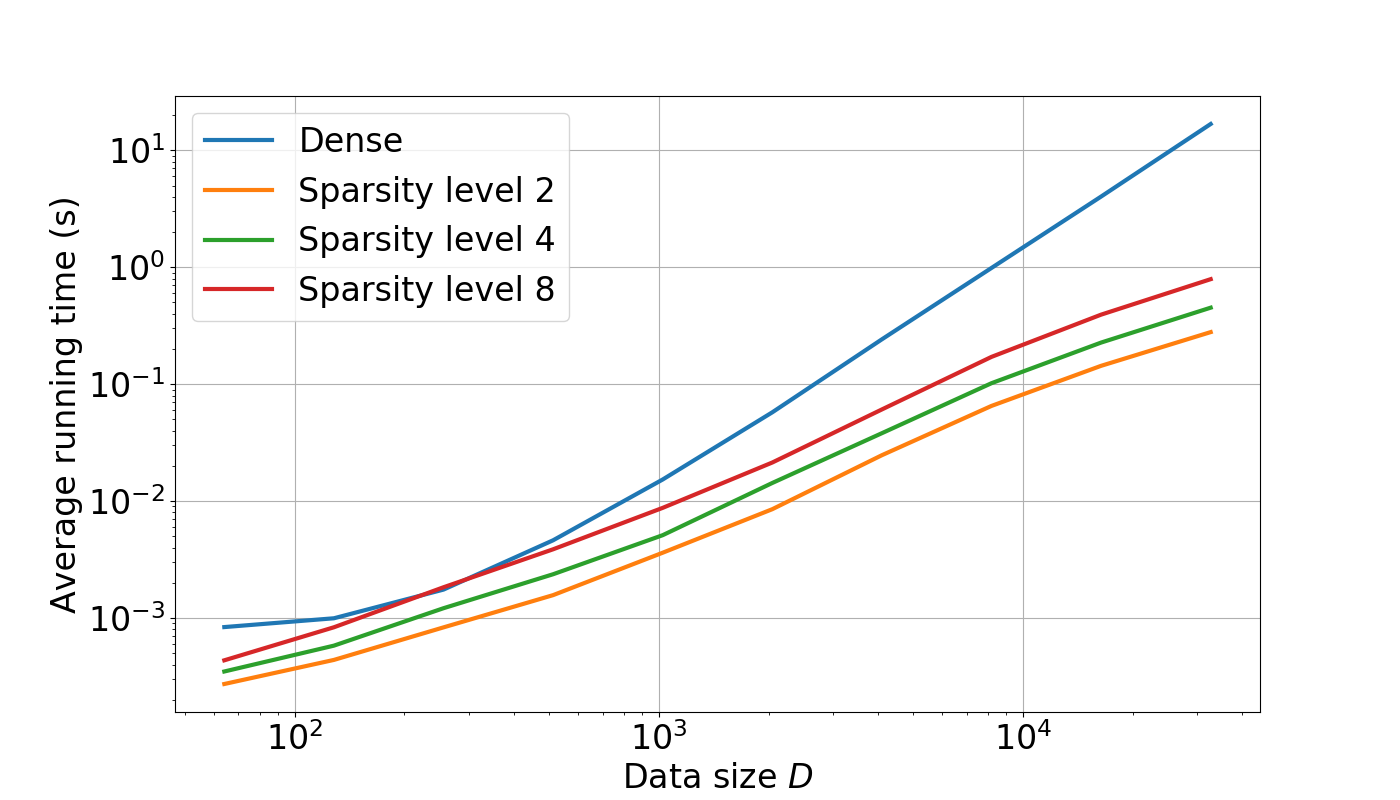
\includegraphics[width=.5\textwidth]{RunningTime4VaryingSparsity.png}
% \caption{Running times, averaged over 30 runs, when applying dense or fast $\datadim \times \datadim$ operators to a set of 100 random vectors. The number of factors in fast operators equals $\log_2\left (\datadim\right )$ and the sparsity level denotes the number of non-zero coefficients per row and per column in each factor.}
% \label{fig:time_csr}
% \end{figure}

%\begin{figure}[tbh]
%\centering
%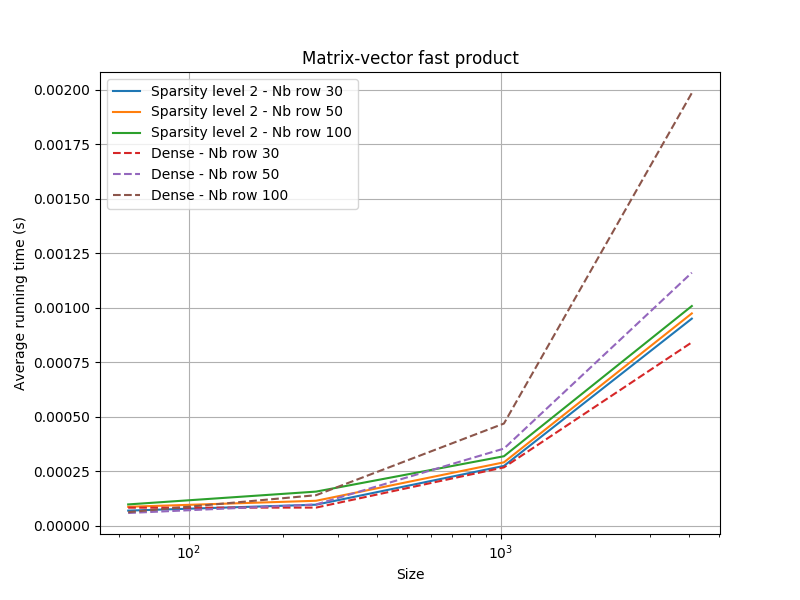
\includegraphics[width=.8\textwidth]{Run_time_sparsity_2.png}
%\caption{Running times, averaged over 30 runs, when applying dense or product of fast operators to a set of 100 random vectors. The number of factors in fast operators equals $\log_2\left (\#~row\right )$ and the sparsity level denotes the number of non-zero coefficients per row and per column in each factor.}
%\label{fig:time_csr_fixed_row_size}
%\end{figure}


\paragraph{Datasets.}
We present results on real-world and toy datasets.
Our experiments are conducted on synthetic and real-world data sets to show (i) --- quantitatively and qualitatively --- the good quality of the obtained centers when using our method on the \texttt{MNIST}~\cite{lecun-mnisthandwrittendigit-2010} and \texttt{Fashion-Mnist}~\cite{Pedregosa2011Scikit} %and \texttt{Labeled Faces in the Wild}~\cite{Huang07e.:labeled} (\texttt{LFW}) 
($D=784$, $K=10$) datasets and (ii) the speed up offered by our method \qkmeans when the number of clusters and the dimensionality of the data are sufficiently large on the \texttt{blobs} synthetic dataset from \texttt{sklearn.dataset}  ($D=2000$, $K=1000$) and the \texttt{Caltech256}~\cite{griffin2007caltech} dataset ($D=2352$, $K=256$) (see supplementary material Section~\ref{supp:datasets} for compact statistics table). \todo[inline]{ne plus faire la distinction entre les datasets pour speedup vs qualité -> retirer les références à blobs qui n'es tplus nécessaire dans ce cas}
%The code of our method \qkmeans is available on request and will be available online soon. \addLG{je serais d'avis de ne pas dire ça mais soit de dire qu'il est déjà disponible, soit de ne rien dire. Sachant qu'on ne peut pas dire qu'il est déjà disponible en ligne avant le processus de reviewing}


\paragraph{Algorithm settings.} 
\qkmeans is used with $Q\eqdef\log_2\left (A\right )$ \todo[inline]{on devrait plutôt utiliser log B sparse factors pour être cohérents avec l'étude théorique -> expériences à re faire} sparse factors, where  $A\eqdef\min\left (\nclusters, \datadim\right )$. 
All factors $\rmS_q$ are with shape $A \times A$ except, depending on the shape of $\rmA$, the leftmost one ($\nclusters\times A$) or the rightmost one ($A\times\datadim$). 
The sparsity constraint of each factor $\rmS_q$ is set in $\mathcal{E}_q$ and is governed by a global parameter denoted as \textit{sparsity level}, which indicates the desired number of non-zero coefficients in each row and in each column of $\rmS_q$. 
Since the projection onto this set of structured-sparsity constraints may be computationally expensive, this projection is relaxed in the implementation of \palm and only guarantees that the number of non-zero coefficients in each row and each column is at least the sparsity level, as in~\cite{LeMagoarou2016Flexible}.
The actual number of non-zero coefficients in the sparse factors is measured at the end of the optimization process and reported in the results.
%The sparse factors are updated using the \palm rather than its hierarchical version, since we observed that this was a better choice in terms of computational cost, with satisfying approximation results (See Figure~\ref{fig:mnist:objfun}~and~\ref{fig:fmnist:objfun}).
Additional details about \palm are given in supplementary material Section~\ref{sec:app:palm4msa}.
The stopping criterion of \kmeans and \qkmeans consists of a tolerance set to $10^{-6}$ on the relative variation of the objective function and a maximum number of iterations set to 10. 
The same principle governs the stopping criterion of \palm with a tolerance set to $10^{-6}$ and a maximum number of iterations set to 300. Each experiment have been replicated using different seed values for random initialisation. 
Competing techniques share the same seed values, hence share the same initialisation of centers as they are sampled uniformly from the dataset. For the \qkmeans experiments, the inital matrix of centroids is processed once by the \textit{Hierarchical}-\palm euristic proposed in \cite{LeMagoarou2016Flexible} but then the simple \palm algorithm is used inside \qkmeans as it didn't impact much of the performance while saving a lot of time. (See supplementary material Section~\ref{supp:hierarchical} for details).

%\subsection{Sparse factors multiplication}
%
%\subsubsection{Sparse factor object}

%\todo[inline]{Parler ici de la configuration de \qkmeans: $Q\eqdef\log_2\left (A\right )$, critère d'arrêt (nombre d'itération, tolérance), ordre des mises à jours, palm4msa plutôt que la version hiérarchique, taille des matrices $\rmS_q$, scaling coefficient, définition de 	$\mathcal{E}_q$.
%}

\subsection{Clustering}

\begin{figure*}[h]
\begin{subfigure}[b]{.49\textwidth}
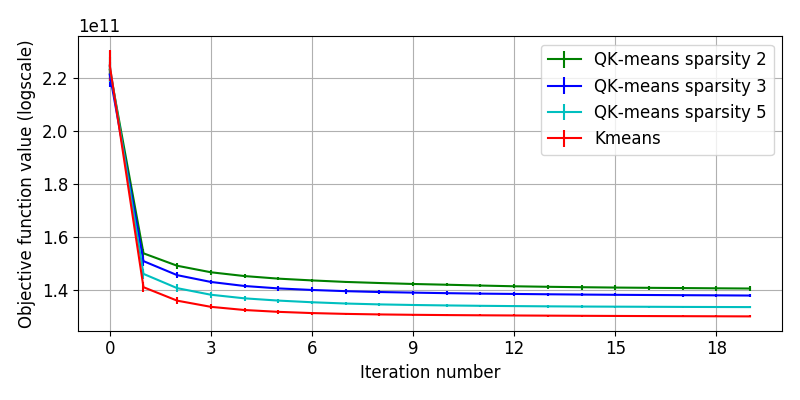
\includegraphics[width=\textwidth]{mnist30_objective.png}
\caption{MNIST, $\nclusters=30$: objective function.}
\label{fig:mnist:objfun}
\end{subfigure}
\begin{subfigure}[b]{.49\textwidth}
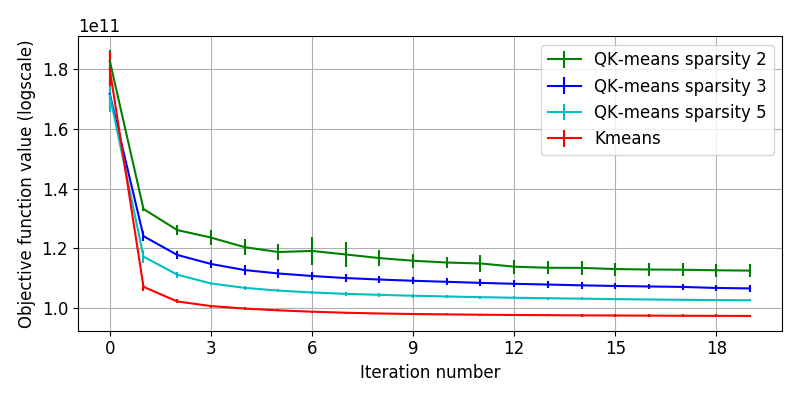
\includegraphics[width=\textwidth]{fashmnist30_objective.png}
\caption{Fashion-MNIST, $\nclusters=30$: objective function.}
\label{fig:fmnist:objfun}
\end{subfigure}
\begin{subfigure}[t]{.49\textwidth}
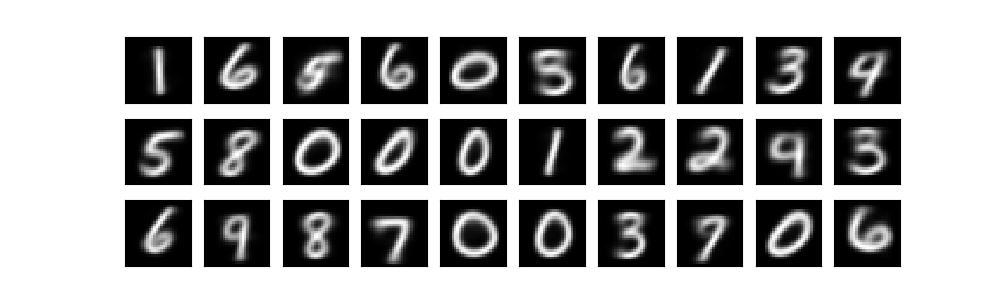
\includegraphics[width=\textwidth]{mnist30_kmeans_centroids.png}
\caption{\kmeans centers.}
\label{fig:mnist:kmeans:centers}
\end{subfigure}
\begin{subfigure}[t]{.49\textwidth}
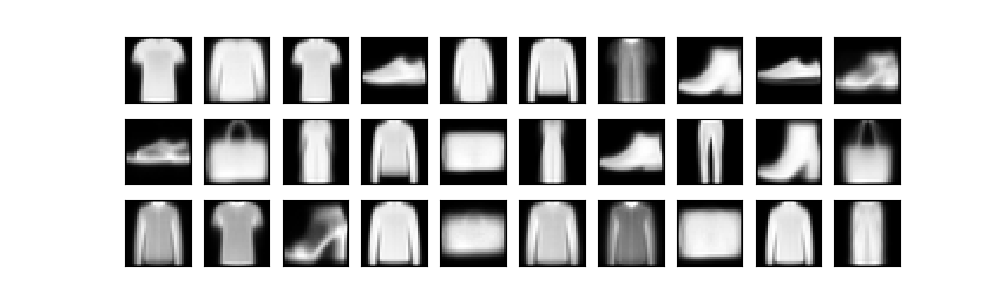
\includegraphics[width=\textwidth]{fashmnist30_kmeans_centroids.png}
\caption{\kmeans centers.}
\label{fig:fmnist:kmeans:centers}
\end{subfigure}
\begin{subfigure}[t]{.49\textwidth}
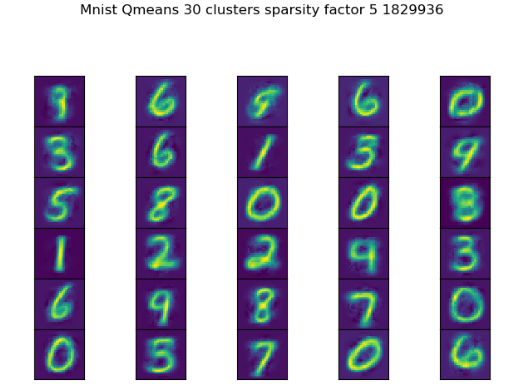
\includegraphics[width=\textwidth]{mnist30_qkmeans_centroids.png}
\caption{\qkmeans centers.}
\label{fig:mnist:qkmeans:centers}
\end{subfigure}
\begin{subfigure}[t]{.49\textwidth}
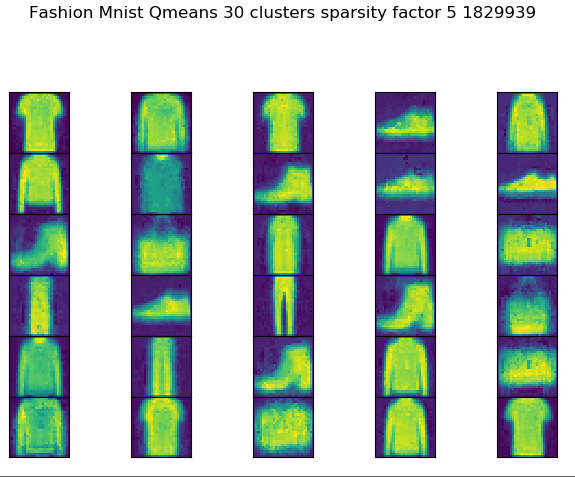
\includegraphics[width=\textwidth]{fashmnist30_qkmeans_centroids.png}
\caption{\qkmeans centers.}
\label{fig:fmnist:qkmeans:centers}
\end{subfigure}
% \begin{subfigure}[t]{.49\textwidth}
% 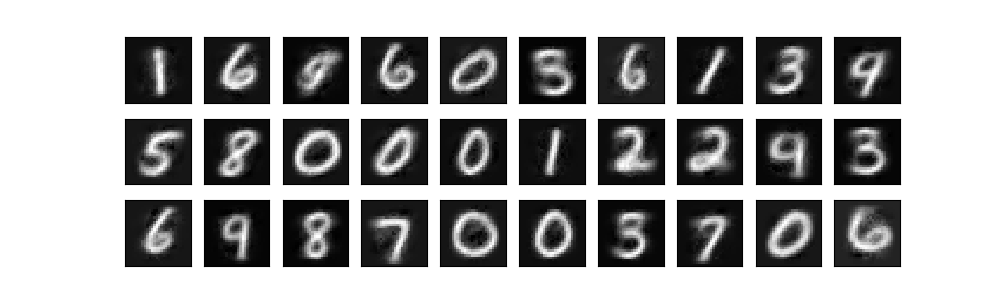
\includegraphics[width=\textwidth]{mnist30_hqkmeans_centroids.png}
% \caption{Hierarchical-\palm \qkmeans centers.}
% \label{fig:mnist:hqkmeans:centers}
% \end{subfigure}
% \begin{subfigure}[t]{.49\textwidth}
% 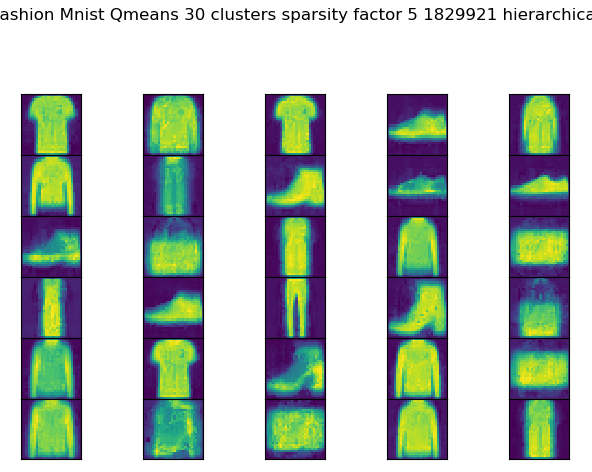
\includegraphics[width=\textwidth]{fashmnist30_hqkmeans_centroids.png}
% \caption{Hierarchical-\palm \qkmeans centers.}
% \label{fig:fmnist:hqkmeans:centers}
% \end{subfigure}
\caption{Clustering results on MNIST (left) and Fashion-MNIST (right) for $\nclusters=30$ clusters.}
\label{fig:clustering:realdata}
\end{figure*}

\paragraph{Approximation quality.} One important question is the ability of the fast-structure model to fit arbitrary data.
Indeed, no theoretical result about the expressivity of such models is currently available.
In order to assess this approximation quality, the MNIST and Fashion-MNIST data have been clustered into $\nclusters=30$ clusters by \kmeans and \qkmeans with several sparsity levels.
Results are reported in Figure~\ref{fig:clustering:realdata}.
In Figures~\ref{fig:mnist:objfun} and~\ref{fig:fmnist:objfun}, one can observe that the objective function of \qkmeans is decreasing in a similar way as \kmeans over iterations.
In particular, the use of the fast-structure model does not seem to increase the number of iteration necessary before convergence.
At the end of the iterations, the value of objective function for \qkmeans is slightly above that of \kmeans.
As expected, the sparser the model, the more degradation in the objective function.
However, even very sparse models do not degrade the results significantly. %These Figures also demonstrate the convergence property of the \qkmeans algorithm when using the standard, proved convergent, \textit{Palm4MSA} algorithm: the objective function is always non-increasing.
The approximation quality can be assessed visually, in a more subjective and interpretable way, in Figures~\ref{fig:mnist:kmeans:centers} to~\ref{fig:fmnist:hqkmeans:centers} where the obtained centers are displayed as images.
Although some degradation may be observed in some images, one can note that each image obtained with \qkmeans clearly represents a single visual item without noticeable interference with other items.

\paragraph{Clustering assignation times.}
Higher dimensions are required to assess the computational benefits of the proposed approach, as shown here with the comparison between the \texttt{MNIST} dataset and the others: the \texttt{MNIST} dataset has low dimensionality and low cluster number then the vector assignation times are even worse due to the computational overload induced by our poor implementation. 
Results reported in Table~\ref{tab:results} show that in this setting and with the current implementation, the computational advantage of \qkmeans is observed in high dimension, for $\nclusters=256$ and $\nclusters=512$ clusters. It is worth noticing that when $K$ increases, the running times are not affected that much for \qkmeans while it significantly grows for \kmeans. These trends are directly related to the number of model parameters that are reported in the figure. It can be noticed that these numbers of parameters doesn't necessarily grow with the number of clusters because each sparse factor must have \textit{at least} a given number of value for each line and each column of the sparse factor, in this case 2. 
\todo[inline]{a retirer vu que les bénéfices en flop sont sensibles indépendamment de la dimension}


%\todo[inline]{Montrer ensuite les temps d'assignation en mode batch 5000 sur blobs, cf. Figure~\ref{fig:clustering:blobs:assignation_time}. Objectif: montrer qu'à partir d'une certaine dimension, \qkmeans est plus rapide.}
%on-line\footnote{Anonymous URL.}.

% \begin{figure}[tbh]
% \centering
% 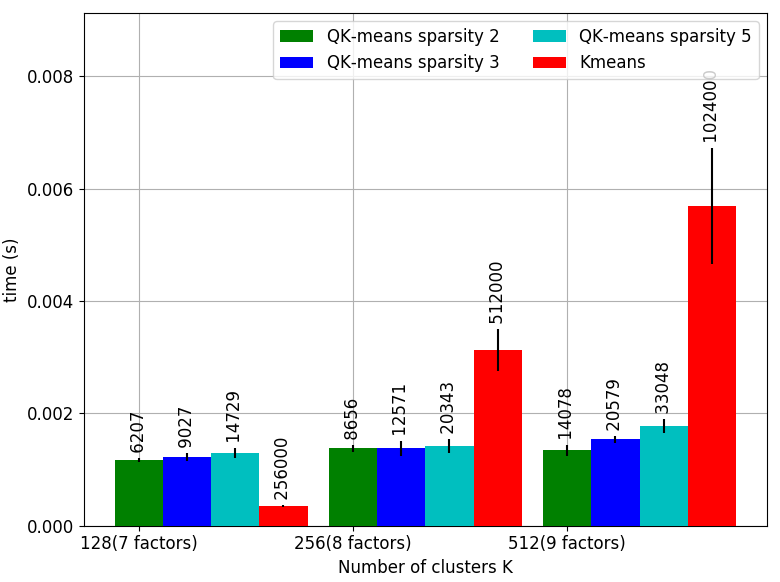
\includegraphics[width=.45\textwidth]{blobs_assignation_time.png}
% \caption{Clustering Blobs data: running times of the assignation step, averaged over 5 runs. The vertical black lines are the standard deviation w.r.t. the runs and the average number of parameters actually learned  in the models are reported above those lines.\addVE{to be completed}.}
% \label{fig:clustering:blobs:assignation_time}
% \end{figure}

% No experiments shows the runtime improvement of the \qkmeans algorithm compared to the \kmeans one but supplementary material Section~\ref{supp:traintime_expe} shows preliminary results on this matter.


\subsection{Nearest-neighbor search in a large dataset}
The Nearest-neighbor search is a fundamental task that suffers from computational limitations when the dataset is large.
Fast strategies have been proposed, e.g., using kd trees or ball trees.
One may also use a clustering strategy to perform an approximate nearest-neighbor search: the query is first compared to $\nclusters$ centers computed beforehand by clustering the whole dataset, and the nearest neighbor search is then performed among a lower number of data points, within the related cluster.
We compare this strategy using \kmeans and \qkmeans against the \texttt{scikit-learn} implementation~\cite{Pedregosa2011Scikit} of the nearest-neighbor search (brute force search, kd tree, ball tree).
Inference time results \todo[inline]{pas de resultats de temps (ni de flop) dans ce cas, c'est moins intéressant}and accuracy results are displayed in Table~\ref{tab:results}. 
% As shown in Figure~\ref{fig:nn:blobs:accuracy}, the accuracy of the approximate nearest neighbor search is above $0.99$ \todo{Accuracy $>0.99$ to be checked} for all the tested variants of \qkmeans, which is an solid evidence about the reliability of the approach.
The results for the Brute Force Search, KD Tree and Ball Tree are not available for some dataset because they were longer than 10 times the \kmeans search version in the same setting.
The running times reported in the table show a drastic advantage of using a clustering-based approximate search 
%\todo{to be completed by reporting the actual acceleration ratio obtained by \qkmeans over the three sklearn options.} 
and this advantage is even stronger with the clustering obtained by our \qkmeans method. We see that for the \texttt{Blobs} dataset, this speed-up comes at a cost as we can see a drop in classification performance but not for the other datasets. We believe our method is more sensible to the very noisy nature of the blobs dataset.\todo[inline]{retirer les résultats avec blobs et mettre l'accent sur le fait que les résultats obtenus sont tout aussi bons avec K-means que qk-means}
% 
% \begin{figure}[tbh]
% \centering
% 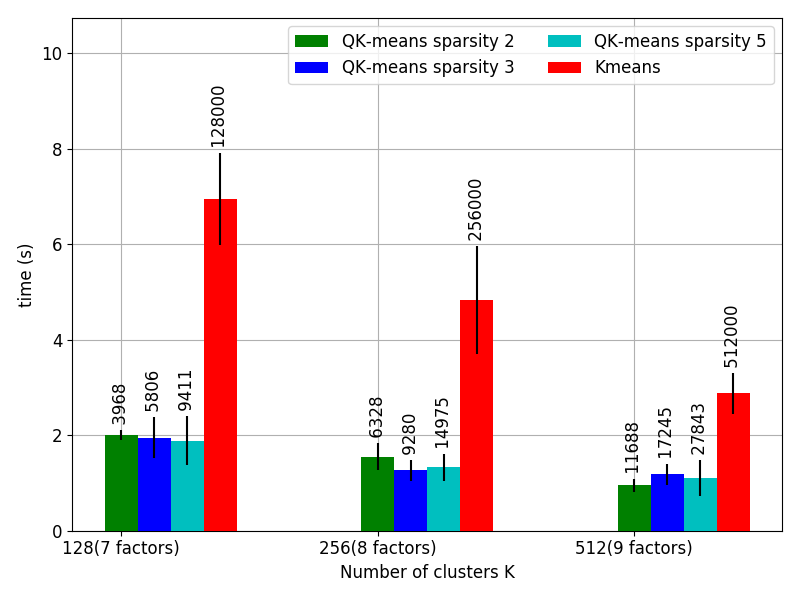
\includegraphics[width=.45\textwidth]{blobs_1nn_inference_time.png}
% \label{fig:nn:blobs:times}
% \caption{Running time of nearest neighbor search on blobs data. Results are averaged over 5 runs (vertical lines: standard deviation) and the average number of parameters actually learned is reported above each bar.}
% \label{fig:nn:blobs}
% \end{figure}


\begin{table*}[!htb]
% \centering
\resizebox{\textwidth}{!}{\begin{tabular}{@{}ccccc|ccc|ccc}
\toprule                                                                                                                                                                             
                                                &                               & \thead{\texttt{Blobs} \\ K=128}       & \thead{\texttt{Blobs} \\ K=256}   & \thead{\texttt{Blobs} \\ K=512}     & \thead{\texttt{Caltech} \\ K=128}       & \thead{\texttt{Caltech} \\ K=256}   & \thead{\texttt{Caltech} \\ K=512}     & \thead{\texttt{MNIST} \\ K=10}   & \thead{\texttt{MNIST} \\ K=16} & \thead{\texttt{MNIST} \\ K=30} \\ 
                                                
\midrule

                                                                                                                                                                                                                                                                             
\multirow{2}{*}{\shortstack{Vector assignation \\ time (ms)}} & \kmeans               & \boldsymbol{$0.3$}                   & $3.1$                                & $5.7$                     & \boldsymbol{$0.2$}                  & \boldsymbol{$1.5$}                    & $4.2$                       & \boldsymbol{$0.003$}           & \boldsymbol{$0.005$}   & \boldsymbol{$0.006$}   \\
                                                              & \qkmeans              & $1.2$                                & \boldsymbol{$1.4$}                 & \boldsymbol{$1.3$}                     & $1.3$                   & \boldsymbol{$1.5$}                    & \boldsymbol{$1.7$}            & $0.5$                       & $0.6$                 & $0.8$   \\

                                                        
\midrule \midrule                                                                                                                                                                                                                                                                                                
                                                        
                                                        

% \multirow{3}{*}{\shortstack{Nyström \\ approximation \\ error}}   & \kmeans               & \boldsymbol{$0.032$}                  & \boldsymbol{$0.030$}                   & \boldsymbol{$0.027$}           & \boldsymbol{$0.6$}                  & \boldsymbol{$0.6$}                   & \boldsymbol{$0.6$}           & \boldsymbol{$0.087$}          & \boldsymbol{$0.069$}        & \boldsymbol{$0.049$}   \\
%                                                         & \qkmeans              & \boldsymbol{$0.032$}                  &  \underline{$0.031$}                  & \underline{$0.029$}             & \boldsymbol{$0.6$}                  & \boldsymbol{$0.6$}                   & \boldsymbol{$0.6$}             & \underline{$0.091$}           & \underline{$0.083$}         & \underline{$0.061$}   \\
%                                                         & Uniform sampling      & $0.035$                               & $0.032$                               & $0.030$                         & \boldsymbol{$0.6$}                  & \boldsymbol{$0.6$}                   & \boldsymbol{$0.6$}                 & $0.184$              & $0.147$            & $0.105$   \\
% 
%                                                         
% \midrule \midrule                                                                                                                                                                                                                                                                 


\multirow{2}{*}{\shortstack{Nyström Inference \\ time (ms)}}    & \kmeans               & \boldsymbol{$0.11$}                   & \boldsymbol{$0.17$}                  & $0.32$                            & \boldsymbol{$0.09$}                  & \boldsymbol{$0.14$}                    & \boldsymbol{$0.21$}                       & \boldsymbol{$0.06$}           & \boldsymbol{$0.06$}   & $0.07$   \\
                                                        & \qkmeans              & $0.13$                                & $0.18$                             & \boldsymbol{$0.22$}                 & $0.24$                               &$0.30$                               & $0.40$            & $0.08$                        & $0.07$                 & \boldsymbol{$0.06$}   \\

                                                        
\midrule \midrule                                                                                                                                                                                                                                                                                                


\multirow{3}{*}{\shortstack{1NN \\ Accuracy}}           & \kmeans               & \boldsymbol{$0.96$}                   & \boldsymbol{$0.97$}                & \boldsymbol{$0.99$}                 & \boldsymbol{$0.11$}                  & \boldsymbol{$0.11$}                    & \boldsymbol{$0.11$}        & \underline{$0.96$}           & \underline{$0.96$}   & \underline{$0.96$}   \\
                                                        & \qkmeans              & $0.61$                                & $0.49$                             & $0.37$                              & $0.10$                               & $0.10$                               & $0.09$                       & \underline{$0.96$}           & \underline{$0.96$}                 & $0.95$   \\
%                                                         & Brute force          &                                           \multicolumn{3}{c|}{$N/A$}                                               &                               \multicolumn{3}{c|}{$N/A$}                                                    &                    \multicolumn{3}{c}{\boldsymbol{$0.97$}}                                 \\
                                                        & Ball-tree            &                                           \multicolumn{3}{c|}{$\text{timed-out}$}                                               &                               \multicolumn{3}{c|}{$\text{timed-out}$}                                                    &                    \multicolumn{3}{c}{\boldsymbol{$0.97$}}                                 \\
%                                                         & Kd-tree              &                                           \multicolumn{3}{c|}{$N/A$}                                               &                               \multicolumn{3}{c|}{$N/A$}                                                    &                    \multicolumn{3}{c}{\boldsymbol{$0.97$}}                                 \\

                                                        
\midrule \midrule                                                                                                                                                                                                                                                                                                
                                                                                                                                                                                                                                                                             
                                                                                                                                                                                                                                                                             
\multirow{3}{*}{\shortstack{1NN \\ Runtime (s)}} & \kmeans               & $17.2$                   & $15.8$                  & $9.5$                & $74.4$                                             & $50.0$                                           & $35.3$                       & \boldsymbol{$0.74$}           & \boldsymbol{$0.83$}   & \boldsymbol{$0.88$}   \\
                                                        & \qkmeans              & \boldsymbol{$5.3$}                                & \boldsymbol{$3.0$}                 & \boldsymbol{$1.2$}             & \boldsymbol{$67.0$}                               & \boldsymbol{$30.9$}                              & \boldsymbol{$19.8$}            & \underline{$0.73$}           & \underline{$0.79$}   & \underline{$0.86$}   \\
%                                                         & Brute force          &                                           \multicolumn{3}{c|}{$N/A$}                                          &                               \multicolumn{3}{c|}{$N/A$}                                                    &                    \multicolumn{3}{c}{$2176.1$}                                 \\
                                                        & Ball-tree            &                                           \multicolumn{3}{c|}{$\text{timed-out}$}                                          &                               \multicolumn{3}{c|}{$\text{timed-out}$}                                                    &                    \multicolumn{3}{c}{$553.0$}                                 \\
%                                                         & Kd-tree              &                                           \multicolumn{3}{c|}{$N/A$}                                          &                               \multicolumn{3}{c|}{$N/A$}                                                     &                    \multicolumn{3}{c}{$707.0$}                                 \\
                                                                                                                                                                                                  
                                                        
\midrule \midrule                                                                                                                                                                                                                                                                                                
                                                                                                                                                                                                                                                                             
                                                                                                                                                                                                                                                                             
\multirow{2}{*}{\shortstack{Nyström + SVM \\ Accuracy}} & \kmeans               & \boldsymbol{$0.98$}                   & \boldsymbol{$1.0$}                  & \boldsymbol{$1.0$}                     & \boldsymbol{$0.16$}                  & \boldsymbol{$0.17$}                    & \boldsymbol{$0.18$}                       & \boldsymbol{$0.74$}           & \boldsymbol{$0.83$}   & \boldsymbol{$0.88$}   \\
                                                        & \qkmeans              & $0.95$                                & \boldsymbol{$1.0$}                 & \boldsymbol{$1.0$}                     & $0.15$                               & $0.16$                               & $0.16$            & $0.73$                       & $0.79$                 & $0.86$   \\

\midrule \midrule                                                                                                                                                                                                                                                      
                                                                                                                                                                                                                                                                             
\multirow{2}{*}{\shortstack{Number of \\parameters}}    & \kmeans               & $256,000$                   & $512,000$                             & $1,024,000$                               & $301,056$                             & $602,112$                              & $1,204,224$                       & $7,840$           & $12,544$   & $25,088$   \\
                                                        & \qkmeans              & $\boldsymbol{6,207}$        & \boldsymbol{$8,656$}                 & \boldsymbol{$14,078$}                     & \boldsymbol{$10,409$}                  & \boldsymbol{$13,846$}                  & \boldsymbol{$21,013$}            & $\boldsymbol{2,610}$    & \boldsymbol{$2,269$}       & \boldsymbol{$2,427$}    \\                                                        
                                                                                    
\bottomrule
\end{tabular}}
\caption{
Results of numerical experiments: average Nyström transformation time for a sample set of size $5000$; 1-nearest neighbor and SVM classification accuracy on top of Nyström transformation on the test set. The \qkmeans results are obtained with sparse factors with at least 2 values in each line/column. Every experiment results are averaged over 5 runs. Best results are bold while second best are underlined (when necessary). ``Ball-tree'' aggregates the results of the ``brute'' and ``kd-tree'' implementations of 1NN from \texttt{sklearn} as it has given the best results of those. The vector assignation time is measured for one vector while the other times are measured for a whole matrix at once (See supplementary material Section~\ref{seq:sparse_factor_benchmarking} for benchmark)}
\label{tab:results}
\end{table*}

\subsection{Nyström approximation}

In this sub-section, we show how we can take advantage of the fast-operator obtained as output of our \qkmeans algorithm in order to speed-up \todo[inline]{pas vraiment un speed-up: lighten plutot}the computation in the Nyström approximation. 
We start by giving background knowledge on the Nyström approximation then we present some recent work aiming at accelerating it using well known fast-transform methods. 
We finally stem on this work to present a novel approach based on our \qkmeans algorithm. \todo[inline]{pourquoi ne pas comparer la qualité dans les deux cas?}

\subsubsection{Background on the Nyström approximation}

Standard kernel machines are often impossible to use in large-scale applications because of their high computational cost associated with the kernel matrix $\rmK$ which has $O(N^2)$ storage and $O(N^2D)$ computational complexity: $\forall i,j \in\intint{\nexamples}, \rmK_{i,j} = k(\rvx_i, \rvx_j)$. A well-known strategy to overcome this problem is to use the Nyström method which computes a low-rank approximation of the kernel matrix on the basis of some pre-selected landmark points. 

Given $K \ll N$ landmark points $\{\rmU_i\}_{i=1}^{K}$, the Nyström method gives the following approximation of the full kernel matrix:
%
\begin{equation}
 \label{eq:nystrom}
 \rmK \approx \tilde\rmK = \rmC\rmW^\dagger\rmC^T,
\end{equation}
%
with $\rmW \in \R^{K \times K}$ containing all the kernel values between landmarks: $\forall i,j \in [\![K]\!]~ \rmW_{i,j} = k(\rmU_i, \rmU_j)$; $\rmW^\dagger$ being the pseudo-inverse of $\rmW$ and $\rmC \in \R^{N \times K}$ containing the kernel values between landmark points and all data points: $\forall i \in [\![N]\!], \forall j \in [\![K]\!]~ \rmC_{i, j} = k(\rmX_i, \rmU_j)$.

\subsubsection{Efficient Nyström approximation}

A substantial amount of research has been conducted toward landmark point selection methods for improved approximation accuracy \cite{kumar2012sampling} \cite{musco2017recursive}, but much less has been done to improve computation speed. In \cite{si2016computationally}, the authors propose an algorithm to learn the matrix of landmark points with some structure constraint, so that its utilisation is fast, taking advantage of fast-transforms. This results in an efficient Nyström approximation that is faster to use both in the training and testing phases of some ulterior machine learning application.

Remarking that the main computation cost of the Nyström approximation comes from the computation of the kernel function between the train/test samples and the landmark points, \cite{si2016computationally} aim at accelerating this step. In particular, they focus on a family of kernel functions that has the form $k(\rvx_i, \rvx_j) = f(\rvx_i) f(\rvx_j) g(\rvx_i^T\rvx_j)$, where $f: \R^D \rightarrow \R$ and $g: \R \rightarrow \R$. They show that this family of functions contains some widely used kernels such as the Gaussian and the polynomial kernel. Given a set of $K$ landmark points $\rmU \in \R^{K \times D}$ and a sample $\rvx$, the computational time for computing the kernel between $\rvx$ and each row of $\rmU$ (necessary for the Nyström approximation) is bottlenecked by the computation of the product $\rmU\rvx$. They hence propose to write the $\rmU$ matrix as the concatenation of structured $S = K / D$ product of matrices such that $\rmU = \left[ \rmV_1 \rmH^T, \cdots, \rmV_S\rmH^T  \right]^T$, where the $\rmH$ is a $D \times D$ matrix associated with a fast transform such as the \textit{Haar} or \textit{Hadamard} matrix, and the $\rmV_i$s are some $D \times D$ diagonal matrices to be either chosen with a standard landmark selection method or learned using an algorithm they provide.

Depending on the $\rmH$ matrix chosen, it is possible to improve the time complexity for the computation of $\rmU\rvx$ from $O(KD)$ to $O(K \log{D})$ (\textit{Fast Hadamard transform}) or $O(K)$ (\textit{Fast Haar Transform}).

\subsubsection{\qkmeans in Nyström}

We propose to use our \qkmeans algorithm in order to learn directly the $\rmU$ matrix in the Nyström approximation so that the matrix-vector multiplication $\rmU \rvx$ is cheap to compute, but the structure of $\rmU$ is not constrained by some pre-defined transform matrix. We propose to take the objective $\rmU$ matrix as the \kmeans matrix of $\rmX$ since it has been shown to achieve good reconstruction accuracy in the Nyström method \cite{kumar2012sampling}.

As shown in the next sub-section, our algorithm allows to obtain an efficient Nyström approximation, while not reducing too much the quality of the \kmeans landmark points which are encoded as a factorization of sparse matrix. 

\subsubsection{Results}

The Table~\ref{tab:results} summarizes the results achieved in the Nyström approximation setting. An histogram representation and an evaluation for other sparsity factors are available in the supplementary material~Section~\ref{supp:nystrom}.

The ``Nyström inference time'' displays the average time for computing one line of the approximated matrix in Equation~\ref{eq:nystrom}\todo[inline]{pas le temps mais les FLOP}. For $K=512$, when the landmark matrix is big enough, we clearly see the speed-up offered using the \qkmeans method on the \texttt{Blobs} dataset. Intringingly, this speed-up is not sensible for the \texttt{Caltech} dataset even though the vector assignation time was still faster.\todo[inline]{a retirer, le gain est toujours sensible}

% The top part shows the approximation error of the Nyström approximation based on different sampling schemes w.r.t. the real kernel matrix. This error is computed by the Froebenius norm of the difference between the matrices and then normalized:
% 
% \begin{equation}
%  error = \frac{||\rmK - \tilde\rmK||_F}{||\rmK||_F}.
% \end{equation}

From a more practical point of view, we show in Table~\ref{tab:results} that the Nyström approximation based on \qkmeans can then be used in a linear SVM and achieve as good performance as the one based on the \kmeans approach.






%{RBF networks}

%Besoin d'éclaircir les liens avec RBF networks

%\subsection{nearest-neighbours}

%Besoin d'éclaircir les liens avec nearest neighbours
